\documentclass{beamer}

% Theme choice:
\usetheme{CambridgeUS}

% Title page details:
\title{GoTalk}
\author{Swasti Mishra \and Shreya \and Sara Mukherjee}
\date{\today}

\begin{document}

% Title frame
\begin{frame}
    \titlepage
\end{frame}

\begin{frame}{IDEA}
GoTalk utilizes WebSockets for a real time client-server connection using Go's concurrency model ; enabling real-time, bidirectional communication.
\end{frame}

\begin{frame}{AIM}
    \begin{itemize}
        \item Learning the language Go
        \item Learning how to establish client server connection using WebSocket and HTTPs
    \end{itemize}
\end{frame}

% Outline frame

\begin{frame}{Outline}
    \tableofcontents
\end{frame}

% Tech Stack frame
\section{Tech Stack}
\begin{frame}{Tech Stack}
    \begin{itemize}
        \item \textbf{Frontend}
        \begin{itemize}
            \item HTML/CSS
            \item JavaScript
            \item Bootstrap/ Tailwind CSS
        \end{itemize}
        \item \textbf{Backend}
        \begin{itemize}
            \item Go (Golang)
            \item Gorilla WebSocket
            \item HTTP server
        \end{itemize}
        \item \textbf{Database}
        \begin{itemize}
            \item MySQL
        \end{itemize}
    \end{itemize}
\end{frame}

% Timeline frame
\section{Timeline}
\begin{frame}{Timeline}
    \begin{block}{Week 1}
        \begin{itemize}
            \item Installation
            \item Basic http server
            \item Websocket integration
        \end{itemize}
    \end{block}
    
    \begin{block}{Week 2}
        \begin{itemize}
            \item Handling messages
            \item Chat history database
            \item User interface
            \item Documentation
        \end{itemize}
    \end{block}
\end{frame}

% Plan of Action frame
\section{Plan of Action}
\begin{frame}{Plan of Action}
    \centering
    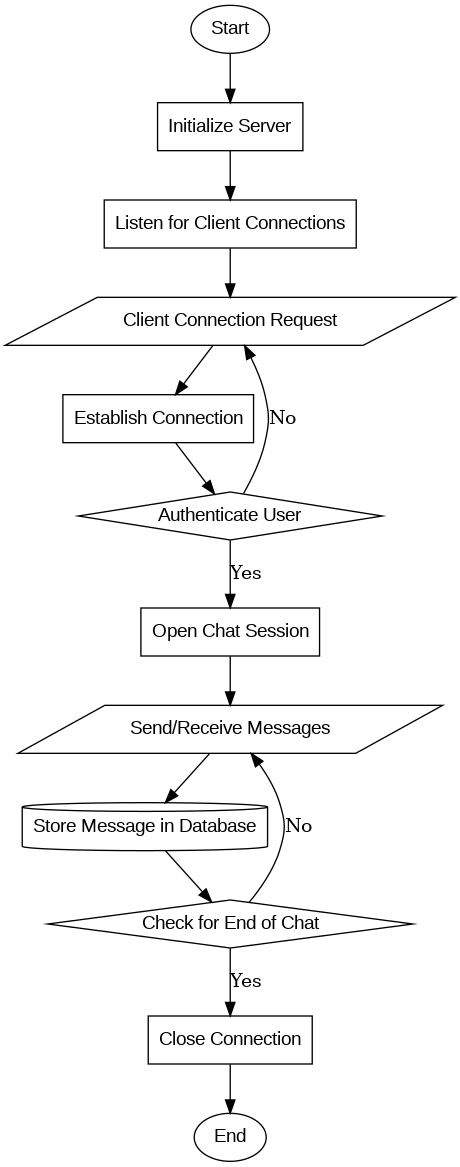
\includegraphics[width=0.25\textwidth]{Graphviz files/Images/graph.png}
\end{frame}

\begin{frame}{Procedure}
    \centering
    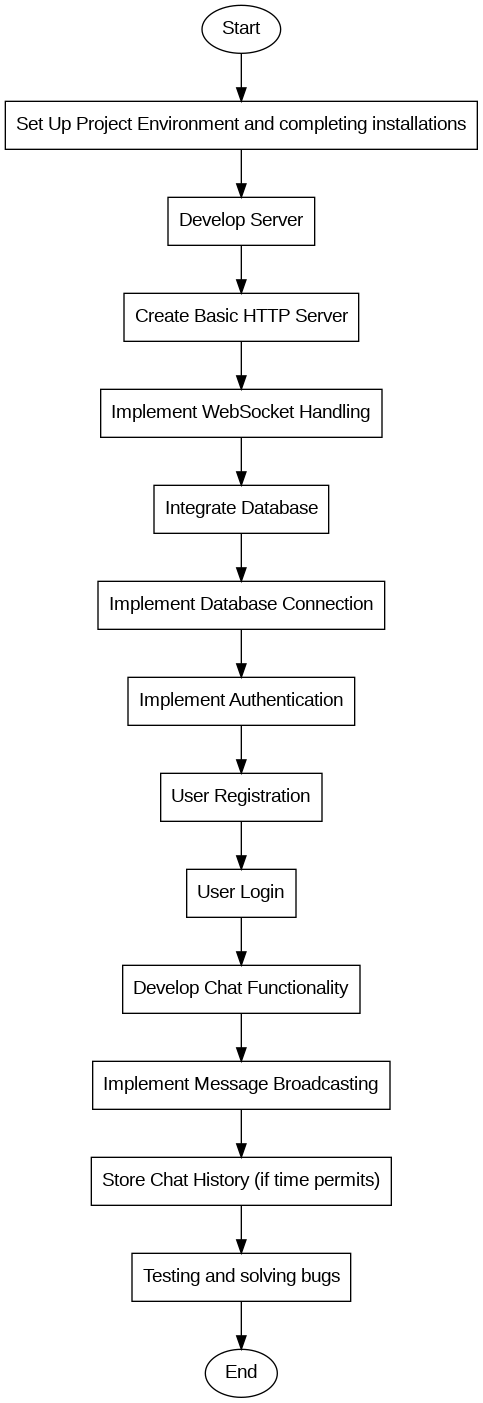
\includegraphics[width=0.22\textwidth]{Graphviz files/Images/implementation.png}
\end{frame}

% Future Scope frame
\section{Future Scope}
\begin{frame}{Future Scope}
    \begin{itemize}
        \item Enhanced UI (file attachment, emojis, etc)
        \item Text Search capabilities
        \item End-to-End Encryption (E2EE)
        \item Polls, community features
        
    \end{itemize}
\end{frame}


% Thank You frame
\begin{frame}{Thank You}
    \centering
    \Huge Thank You!
\end{frame}

\end{document}
